\begin{figure}
\begin{center}
    %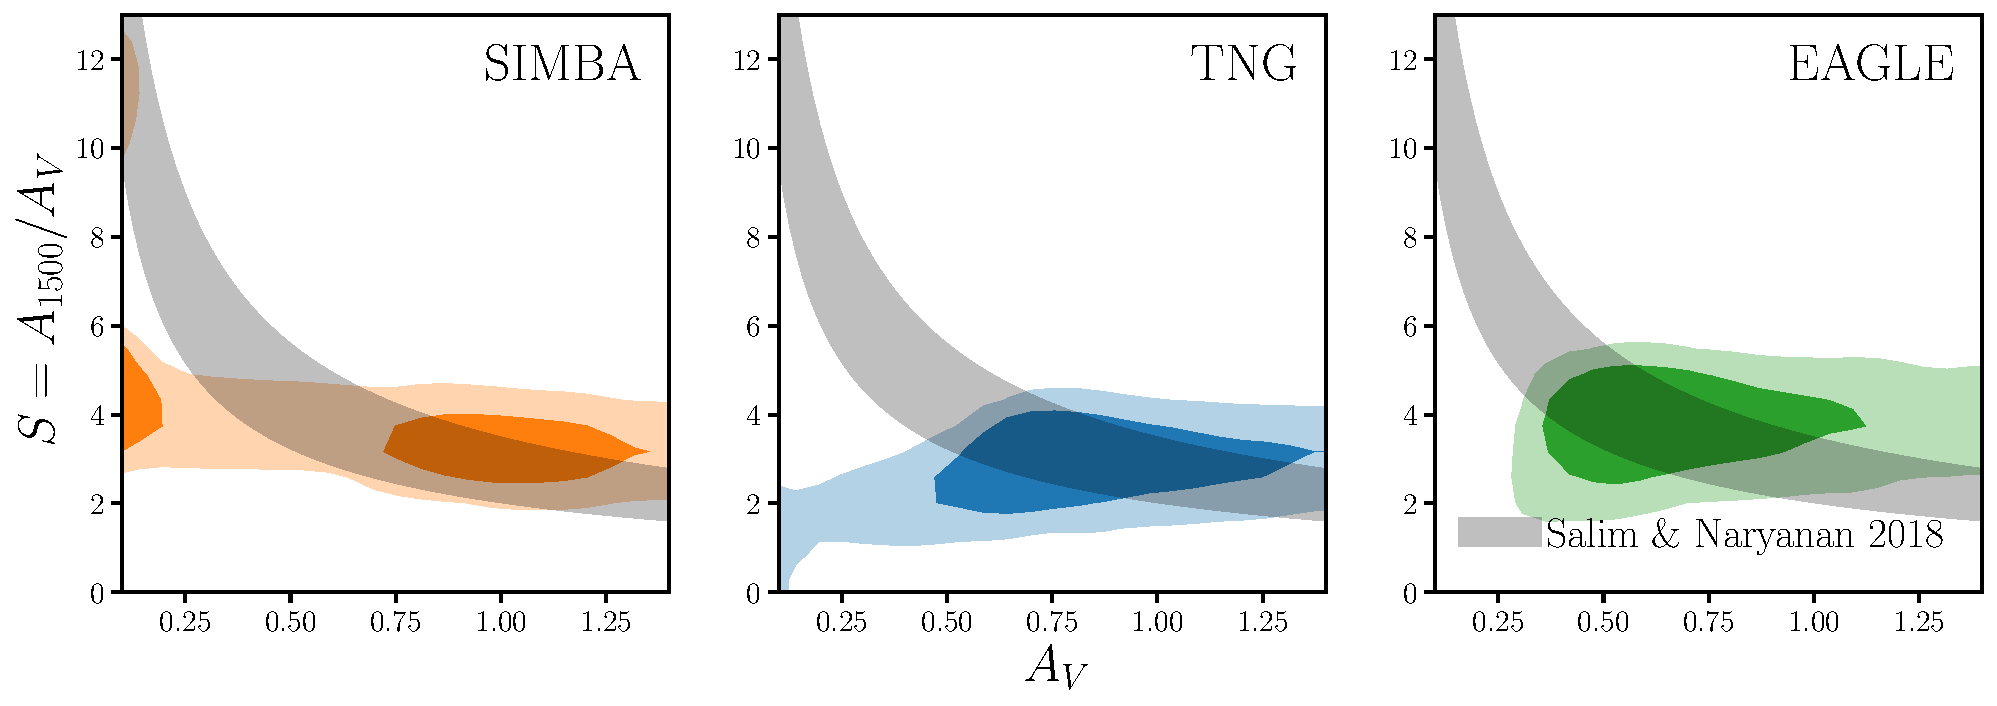
\includegraphics[width=0.4\textwidth]{figs/abc_slope_AV_all.pdf}
    \caption{\label{fig:slope}
    The attenuation-slope relation of the attenuation curves predicted by the
    \eda~model for median posterior parameter values of TNG (blue) and EAGLE
    (green) simulations. We use $A_V$ and $S = A(3000\AA)/A_V$ for attenuation
    and slope, respectively. For comparison, we include the observed 
    attenuation-slope relation from GSWLC2~\citep{salim2020}. We also include 
    the Milky Way (star) and mark the slope of the \cite{calzetti2001} curve
    (dashed). We derived the posteriors of the \eda~model from comparing the
    UV and optical color-magnitude relation and do not fit any observed dust
    attenuation measurements. Yet, using a forward modeling approach, we find 
    excellent agreement between the  attenuation-slope relation predicted by
    the \eda~and observations. 
    }
\end{center}
\end{figure}

\subsection{Reproducing Dust Observations} 
We demonstrated above that we can use the \eda~model in a forward model to
accurately reproduce the observed color-magnitude relations. In the forward
model, the \eda~assigns dust attenuation curves to each simulated galaxy. This
means that we can compare the dust attenuation assigned to the simulated
galaxies (\ie~predicted by the \eda) to the dust attenuation measured from 
observed galaxies. In Figure~\ref{fig:slope}, we present the attenuation-slope 
relation of the \eda~dust attenuation curves for the median posterior parameter 
values of TNG (blue) and EAGLE (green) simulations. For attenuation, we use
$A_V$ and for slope we use the UV-optical slope, $S = A(3000\AA)/A_V$, commonly
found in the literature. To compare with observationss, we include the 
attenuation-slope relations of GSWLC2 galaxies~\citep[grey;][]{salim2020}, the
Milky Way (star), and mark the slope of the \cite{calzetti2001} curve (dashed). 

\emph{The attenuation-slope relation predicted by the \eda~is in excellent 
agreement with observations}. In both the \eda~and observations, galaxies with 
higher attenuation have shallower slopes. The \eda~attenuation curves do not
span the entire range of the observations due to the stellar mass ($M_* \gtrsim 
10^{10} M_\odot$) and luminosity limit ($M_r < -20$) of our sample. Meanwhile, 
the \cite{salim2020} GSWLC2 sample extends down to $M_* \sim 10^{8.5}M_\odot$ 
where they find star-forming galaxies have lower attenuations.  The
attenuation-slope relation is a consequence of the fact that dust scattering 
dominates absoprtion at low attenuation while dust absorption dominates at high 
attenuation~\citep{gordon1994, witt2000, draine2003, chevallard2013}. The
constraints on the \eda~parameters were derived soley from comparing the the
UV and optical color-magnitude relations. This underscores the advantages of 
our forward modeling approach --- without fitting to any dust measurements, we
are able to reproduce the observed properties of dust using the \eda.

\begin{figure}
\begin{center}
    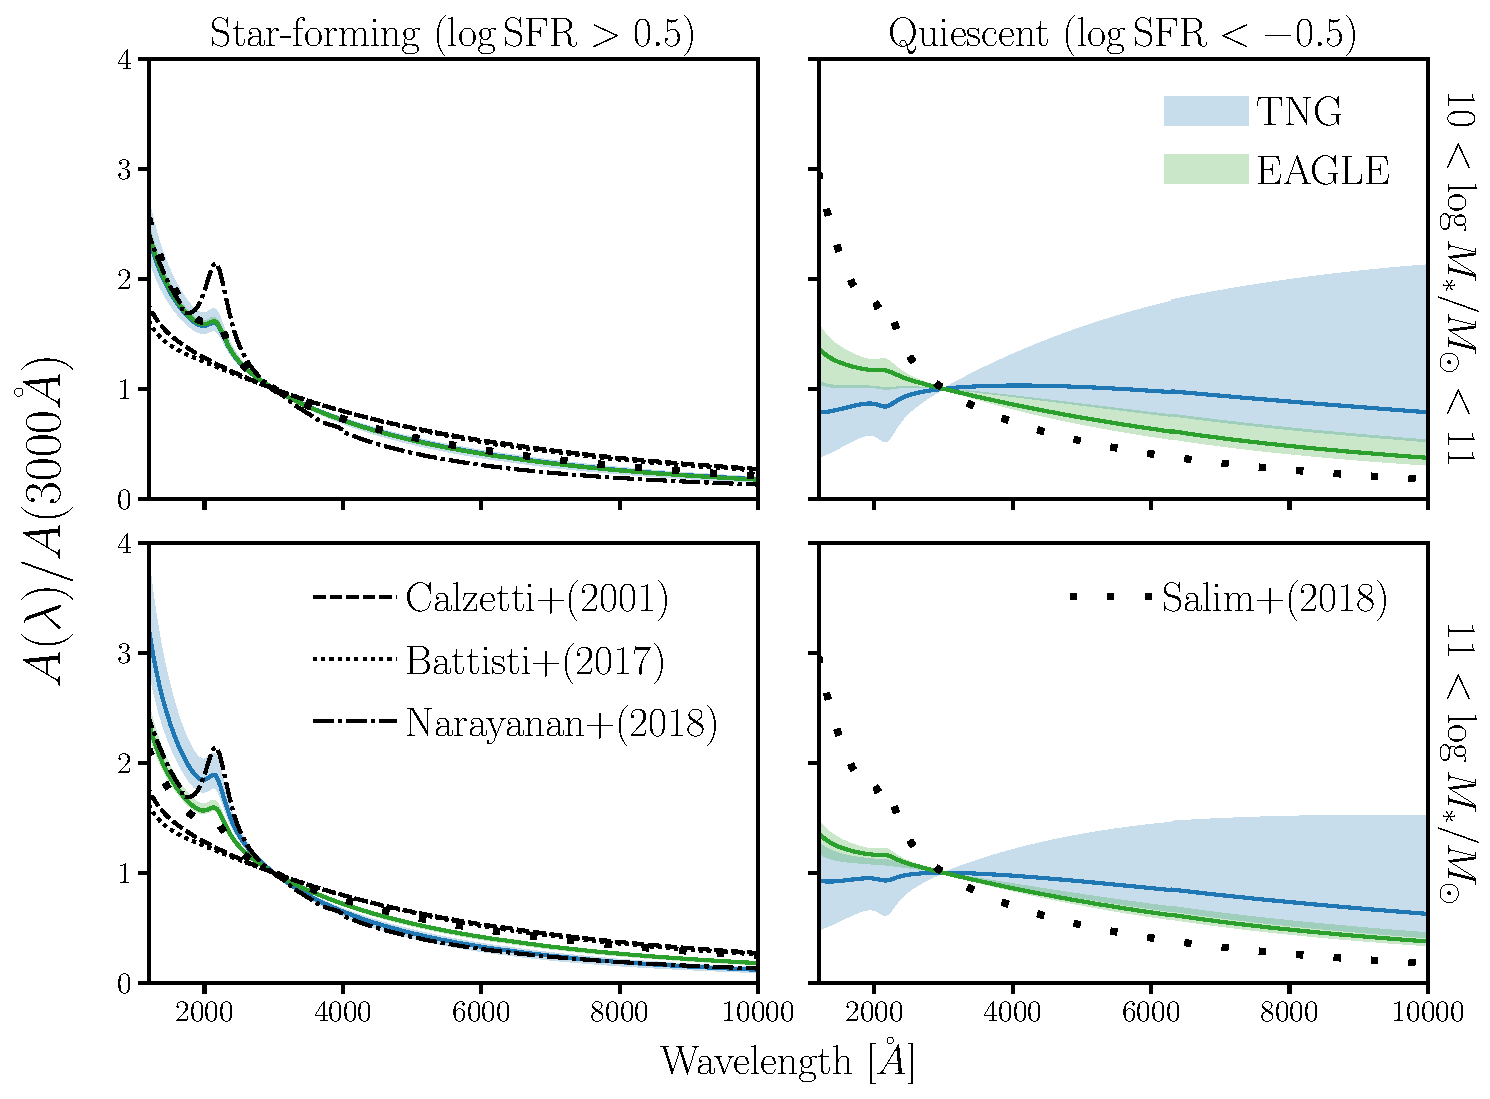
\includegraphics[width=0.85\textwidth]{figs/abc_attenuation.pdf}
    \caption{\label{fig:atten}
    Attenuation curves predicted by the \eda~for median posterior parameter
    values of the TNG (blue) and EAGLE (green) simulations. In the left and
    right panels, we present star-forming and quiescent galaxies classified
    using a $\log {\rm SSFR} = -11$ cut. In the top and bottom panels, we
    present galaxies with $M_* < 10^{11} M_\odot$ and $M_* > 10^{11} M_\odot$,
    respectively. The attenuation curves are normalized at
    $3000\AA$ and we mark the $1\sigma$ standard deviation of the attenuation 
    curves with the shaded region. For comparison, we include
    $A(\lambda)/A(3000\AA)$ measurements from observations~\citep{calzetti2000,
    battisti2017, salim2018} and simulations~\citep{narayanan2018}. 
    For star-forming galaxies, the \cite{calzetti2000} and \cite{battisti2017}
    attenuation curves are shallower than the \eda~attenuation curves, but 
    they probe less massive galaxies than our sample. For \cite{salim2018}, 
    which probe a similar $M_*$ range, we find goood agreement. We also find good agreement with 
    median attenuation curve of star-forming galaxies in \cite{narayanan2018}.
    With \eda, we can also constrain the attenuation curves of quiescent 
    galaxies, which are challenging to directly measure in observations. 
    Quiescent galaxies have significantly shallower attenuation curves than
    star-forming galaxies.
    }
\end{center}
\end{figure}

We can more closely compare the attenuation curves predicted by the \eda~to 
observations. In the left panels of Figure~\ref{fig:atten}, we present the 
attenuation curves of star-forming galaxies predicted by the \eda~model for 
the median posterior parameter values of TNG (blue) and EAGLE (green). In 
the top panel, we present galaxies with $M_* < 10^{11} M_\odot$; in 
the bottom we present galaxies with $M_* > 10^{11} M_\odot$. We define
galaxies with $\log {\rm SSFR} > -11$ as star-forming. The attenuation curves 
are normalized at
$3000\AA$ and we present the variation in the attenuation curves in the shaded
region, 1$\sigma$ standard deviation about the median. For comparison,
we include $A(\lambda)/A(3000\AA)$ from observations: \cite{calzetti2000},
\cite{battisti2017}, and \cite{salim2018}. We also include $A(\lambda)/A(3000\AA)$
measured from the \cite{narayanan2018} simulation. The left panels of
Figure~\ref{fig:raw_atten} is the same as in Figure~\ref{fig:atten}, except
with attenuation curves that are not normalized. The normalized attenuation
curves in Figure~\ref{fig:atten} emphasize the slope while the curves in
Figure~\ref{fig:raw_atten} emphasize the amplitude. 

Based on the \eda, star-forming galaxies have higher dust attenuation at lower
wavelengths. This is driven by both TNG and EAGLE predicting star-forming
galaxies that are bluer than observations in the optical and UV wavelengths
(Figure~\ref{fig:obs}). As a result, the \eda~assigns attenuation curves that
significantly redden star-forming galaxies. This is also why TNG, which
predicts a bluer star-forming population, has slightly higher attenuation. 
In Figure~\ref{fig:raw_atten}, we also find that more massive star-forming
galaxies have higher attenuation. This is because the simulations overpredict 
luminous blue star-forming galaxies, which must be attenuated to reproduce
observations. 

The \eda~attenuation curves for both TNG and EAGLE are in good agreement with the
observed \cite{salim2018} attenuation curves. They are also consistent with the
median curve of \cite{narayanan2018}. We ignore the discrepancies between the
\eda~and \cite{narayanan2018} attenuation curves in the amplitude of UV dust
bump, since we keep the UV bump fixed in the \eda. The \eda attenuation curves 
are noticeably steeper than the \cite{calzetti2000} and \cite{battisti2017} curves. 
These attenuation curves, however, are derived from $M_* < 10^{9.9}M_\odot$ 
star-forming galaxies --- well below our $M_*$ range. %Since we find $\mdeltam < 0$ for both the TNG and EAGLE posteriors, the \eda~attenuation curves are consistent with \cite{calzetti2000} and \cite{battisti2017}. 
Overall, the \eda~predicts attenuation curves that are in good agreement with 
both observations and radiative transfer simulations for star-forming galaxies. 
Again, the fact that we reproduce the detailed dust attenuation curves of star-forming 
galaxies in observations and simulations with the \eda, without fitting for
them, highlights the advantages of a forward modeling approach. 

%At low attenuation, dust scattering dominates absoprtion so the 
%attenuation curve steepens because red light scatters isotropically while blue light
%scatters forward~\citep{gordon1994, witt2000, draine2003}. %, which causes more optical-to-IR light to escape the galaxy than UV light
%At high attenuation dust absorption is dominant and the attenuation curve is
%shallower~\citep{chevallard2013}. For the $A_V$ range probed by the DEM, the
%$A_V$--slope relation is in good agreement with GSWLC2 galaxies~\citep[black shaded][]{salim2020}.
%They are also consistent with \cite{leja2017}. We also compare our results to
%theoretical predictions from radiative transfer models, \cite{inoue2005}
%(dotted), the radiative transfer models considered in \cite{chevallard2013}
%(dot dashed), and \cite{trayford2020} (light shaded), which all predict shallower 
%attenuation curves than observations. This is also the case for the
%\cite{narayanan2018} attenuation curves (not included). 
%\emph{The attenuation curve slopes from the DEM for are in excellent
%agreement with observations and better reproduces the observed
%attenuation--slope relation than radiative transfer models.}
